%LaTex cheat sheet template
\documentclass[12pt,a4paper,landscape]{article}

\usepackage{xfrac}
\usepackage[utf8]{inputenc}
\usepackage{amsmath}
\usepackage{amsfonts}
\usepackage{amssymb}
% \usepackage{polynom}
\usepackage{multicol}
\usepackage{geometry}
\usepackage{lipsum}
\usepackage{titlesec}
\usepackage[nodisplayskipstretch]{setspace}
\usepackage{enumitem}
\usepackage{wrapfig}
\usepackage{float}
\usepackage{needspace}
\usepackage{xcolor}

\geometry{a4paper, left=0mm, top=0mm, right=0mm, bottom=1mm}

\titlespacing{\section}{0pt}{0pt}{0pt}
\titlespacing{\subsection}{0pt}{0pt}{0pt}
\titlespacing{\subsubsection}{0pt}{0pt}{0pt}

\setlength{\abovedisplayskip}{0pt}
\setlength{\belowdisplayskip}{0pt}
\setlength{\parindent}{0pt}

\newcommand{\dropsign}[1]{\smash{\llap{\raisebox{-.5\normalbaselineskip}{$#1$\hspace{2\arraycolsep}}}}}

\begin{document}
\begin{multicols*}{2}

    \section*{Formulaire SignProc}
    \subsection*{Introduction to Communication Systems}

\setlength{\intextsep}{0pt}
\begin{figure}[H]
    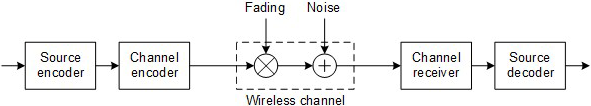
\includegraphics[width=\linewidth]{images/wireless_channel_model.png}
\end{figure}
\textbf{Source encoder:}

Réduit la quantité de données à transmettre ou à stocker, tout en préservant la qualité de
l'information.
Deux types de codage de source, selon que l'on accepte ou non une
perte d'information:

\underline{Lossless coding}: permet de reconstruire exactement les données d'origine à
partir des données codées. Exemples : codage de Huffman, codage arithmétique, codage Lempel-Ziv.

\underline{Lossy coding}: introduit une dégradation irréversible de l'information, mais permet
d'obtenir des taux de compression plus élevés. Exemples : codage par transformée,
codage par quantification vectorielle, codage par prédiction linéaire.

Deux critères pour évaluer la performance d'un codage de source:

\underline{Taux de compression}: rapport entre la quantité de données d'origine et la
quantité de données codées. Plus il est élevé, plus le codage est efficace.

\underline{Distorsion}: mesure de la différence entre les données d'origine et les données
reconstruites. Plus elle est faible, plus le codage est fidèle.

\textbf{Channel encoder:}

Permet de protéger les données contre les erreurs de transmission en ajoutant de la redondance.
Deux types principaux de codage de canal:

\underline{Codage en bloc}: Consiste à diviser les données en blocs de taille fixe et à ajouter
des bits de parité pour détecter et corriger les erreurs.

\underline{Codage Convolutif}: Consiste à appliquer une fonction de transfert aux données en
tenant compte des bits précédents et à générer des bits de contrôle pour détecter et
corriger les erreurs.

\textbf{Wireless channel:}

Support physique qui permet de transmettre les signaux entre l'émetteur et le récepteur.
Il peut être filaire (câble coaxial, fibre optique, etc.) ou sans fil (ondes radio, infrarouge,
etc\dots). Le canal de communication est caractérisé par sa bande passante, qui est la gamme
de fréquences qu'il peut transmettre, et son atténuation, qui est la diminution de l'amplitude
des signaux au cours de la propagation.

Il est imparfait et introduit des perturbations qui altèrent les signaux transmis :

\underline{Bruit}: Variation aléatoire du signal.

\underline{Distorsion}: Modification de la forme du signal.

\underline{Interférence}: Superposition de signaux indésirables.

Les perturbations peuvent entraîner des erreurs de transmission, c'est-à-dire des différences
entre le signal émis et le signal reçu. Pour limiter les erreurs de transmission,
on utilise des techniques de codage, qui consistent à ajouter de l'information redondante
au signal, et de modulation, qui consistent à adapter le signal à la bande passante du canal.

    \subsection*{Source Coding}
\textbf{Information:}

Mesure de l'incertitude ou du désordre d'un système. Plus il y a
d'incertitude, plus il y a d'information. L'information se mesure en bits.

\underline{La mesure d'information:}

apportée par un évenement: $I(E) = -\log_2(P(E))[\text{bits}]$.

\textbf{Entropy:}

Quantité moyenne d'information contenue dans un message. Elle dépend
de la probabilité des symboles du message et de leur indépendance. L'entropie maximale
est atteinte quand tous les symboles sont équiprobables et indépendants.

\underline{La moyenne de l'information:}

(ou hentropie) $H$ envoyée par une source $S$ de $n$ symboles
$X_i$ avec une probabilité $p_i$ est:
$H(S) = -\sum_{i=1}^{n}p_i\cdot\log_2(P(X_i))[\text{bits}]$.

\textbf{Huffman Coding:}

Algorithme qui permet de compresser des données en utilisant
un code binaire variable, adapté à la fréquence d'apparition des symboles.

\setlength{\intextsep}{-5pt}
\begin{wrapfigure}{r}{0.3\textwidth}
    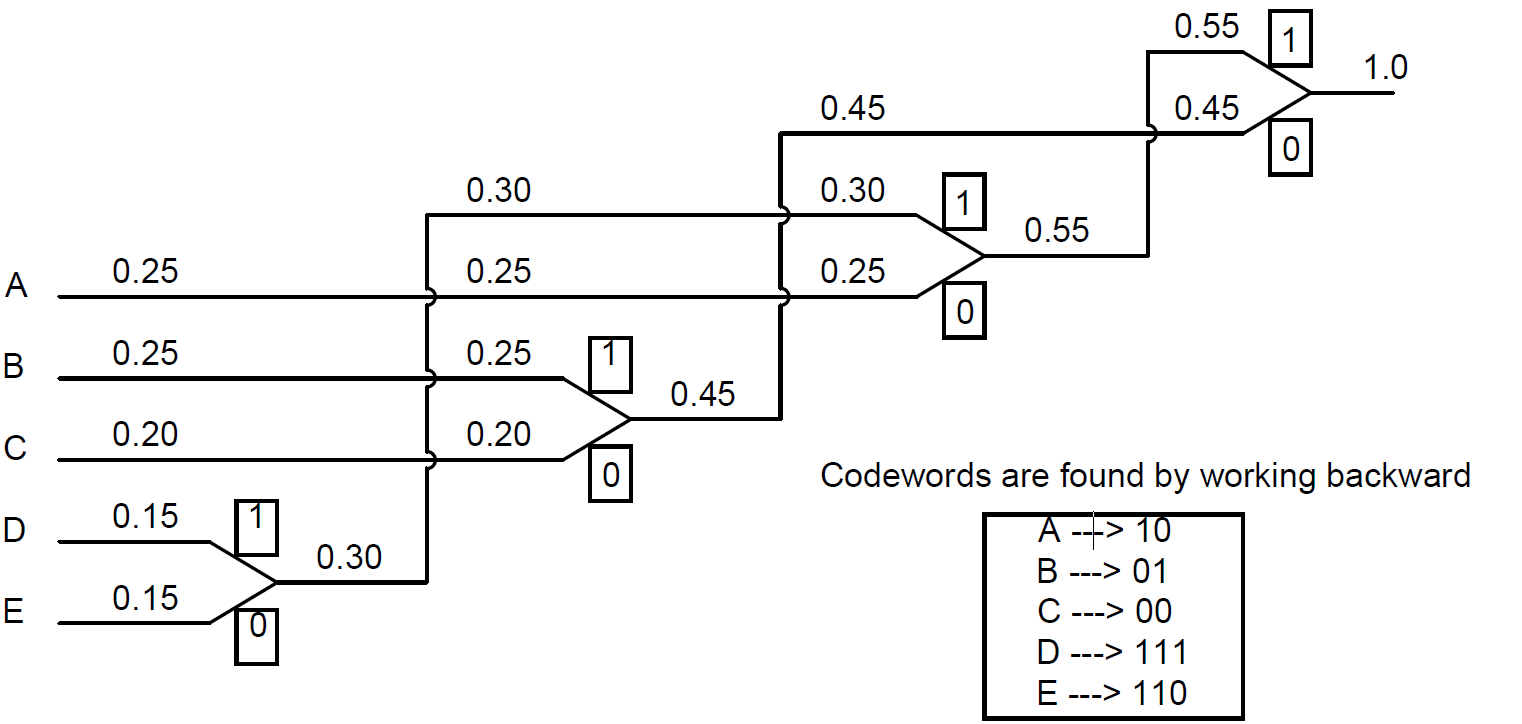
\includegraphics[width=\linewidth]{images/arbre_huffman.png}
\end{wrapfigure}
\underline{Construction de l'arbre de Huffman:}

Extraire les deux nœuds de plus faible
priorité de la file, les fusionner en un nouveau nœud dont la fréquence est la somme
des deux, et l'insérer dans la file, jusqu'à ce qu'il ne reste qu'un seul nœud dans
la file, qui est la racine de l'arbre.

\textbf{Lempel-Ziv Coding:}

Algorithme de compression sans perte qui utilise un
dictionnaire dynamique pour coder les données. Le principe est de remplacer les
séquences répétées par des références au dictionnaire.

\underline{L'algorithme de Lempel-Ziv}:

Chaque mot du dictionnaire va être séparé entre
un préfixe et son dernier bit, au lieu de transmettre le préfixe, on va transmettre
son numéro d'apparition dans le dictionnaire (sous forme binaire) plus le dernier
bit qui sera appelé bit d'innovation. $S = 000101110010100101$
\setlength{\intextsep}{0pt}
\begin{figure}[H]
    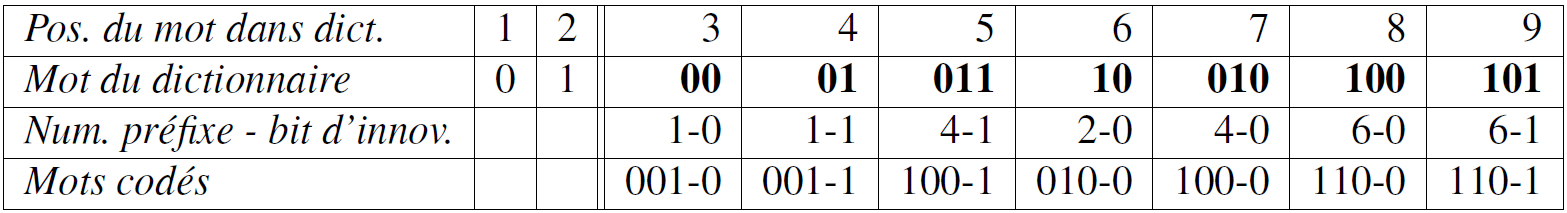
\includegraphics[width=\linewidth]{images/lempel-ziv_table.png}
\end{figure}

\underline{Taille moyenne d'un code:}

envoyé par une source utilisant $l_i$ bits pour chaque symboles :
$\overline{L}=\sum_{i=1}^{n}p_i\cdot l_i[\text{bits par symboles}]$.

\underline{Efficacité d'un code:}

$\text{eff}=\frac{H(S)}{\overline{L}}$.




    \subsection*{Information and Signals}
\textbf{Nomenclature:}

\underline{Signal power}: $S$ [W]

\underline{Bandwidth}: $B$ [Hz]

\underline{Noise power}: $N$ [W]

\underline{Bit energy}: $E_b$ [J]

\underline{Noise spectral density}: $N_0=-174[\text{dBm}]$ [W/Hz]

\underline{Transmission channel capacity}: $C$ [bits/s]

\underline{Transmission speed}: $R$ [bits/s]

\underline{Total number of distinct modulation states}: $M$

\underline{La dégradation due au récepteur}: $NF$

\textbf{Signal:}

\underline{AWGN} (additive white Gaussian noise) est un modèle de bruit.
\begin{figure}[H]
    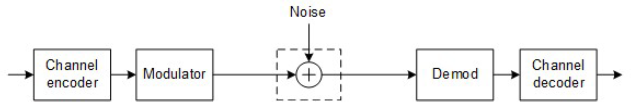
\includegraphics[width=\linewidth]{images/awgn_channel_model.png}
\end{figure}
\underline{Puissance en dBm}: $P_{dBm} = 10\log_{10}\left(\frac{P}{1mW}\right)$

\underline{Noise power}: $N = N_0B$

\underline{Channel capacity}: $C = B\log_2\left(1+\frac{S}{N}\right)$

\underline{Signal power}: $S = E_bR$

\underline{Rendement}: $\frac{E_b}{N_0}=\frac{2^{\sfrac{C}{B}}-1}{\sfrac{R}{B}}$

\underline{BER}: $\frac{1}{2}\cdot\text{erfc}\left(\sqrt{\frac{E_b}{N_0}}\right)$

\textbf{Information:}

L'alphabet numérique est fait de 0 et 1 avec des probabilités
égales $P(0) = P(1)$. Le niveau zéro (0V) est inadapté pour le symbole 0. On attribue
donc 1 au symbole 1 et -1 au symbole 0.

Bit d'information peut être un symbol électrique de forme variable.
Un signal Gaussien est un symbol idéal, c'est une Gaussienne en temps et fréquence.
Plus la Gausienne est étroite en temps, plus le signal est large en fréquence et
vice-versa. L'espacement des symboles est limité par la durée de l'impulsion et
donc par la bande passante $B$

\underline{Nombre de symbols par unité de temps:} $R_b \leq 2B[\sfrac{\text{symbol}}{s}\text{ ou bauds}]$

L'interférence Inter Symbol (ISI) est causée par le dépassement de cette limite.

Un signal numérique doit être filtré passe-bas pour limiter sa bande passante.
Un canal fréquentiel optimal serait un $rect()$, dont la transformée de Fourier inverse
est un $sinc()$. Le pulse en $sinc()$ est théoriquement optimal, mais pratiquement

\setlength{\abovedisplayskip}{-5pt}
\setlength{\belowdisplayskip}{-5pt}
\begin{wrapfigure}{l}{11cm}
    \begin{equation*}
        P(f)=\begin{cases}
            T_S                                                                                                       & \text{si } 0<|f| < \frac{1-\alpha}{2T_S}                       \\
            \frac{T_S}{2}\left[1+\cos\left(\frac{\pi T_S}{\alpha}\left(|f|-\frac{1-\alpha}{2T_S}\right)\right)\right] & \text{si } \frac{1-\alpha}{2T_S} < |f| < \frac{1+\alpha}{2T_S} \\
            0                                                                                                         & \text{sinon}
        \end{cases}
    \end{equation*}
\end{wrapfigure}
inviable, car il nécessite un filtre d'ordre très élevé et il est sensible aux erreurs
temporelles qui créent de l'ISI.
On préfère donc utiliser un \underline{quadrant de sinus (raised cosine)}: $p(t) = \frac{\sin(\sfrac{\pi t}{T_S})}{\sfrac{\pi t}{T_S}}\cdot\frac{\cos(\sfrac{\alpha\pi t}{T_S})}{1-(\sfrac{\alpha t}{T_S})^2}$

Le roll-off factor $\alpha$ permet de contrôler la bande passante du signal.

\underline{Débit binaire}: $R_b = \frac{2B}{1+\alpha}$.

On souhaite filtrer à l'émission pour respecter le canal RF mais aussi à la réception
pour retrouver le signal d'origine après passage dans le canal. Une solution est de
séparer le filtre RC en deux par deux filtres RRC (Root Raised Cosine) un à l'émission et
un à la réception.

\underline{Priorité du filtre RRC}: $\left|H_{rc}(f)\right|=\sqrt{\left|H_{rrc}(f)\right|}\cdot\sqrt{\left|H_{rrc}(f)\right|}=\left|H_{rrc}(f)\right|\cdot \left|H_{rrc}(f)\right|$.
    \subsection*{Channel Coding}
\underline{Produit scalaire de deux vecteur binaires $\overrightarrow{u}$ et $\overrightarrow{v}$}:

$\langle \overrightarrow{u},\overrightarrow{v}\rangle = u_1v_1\bigoplus u_2v_2\bigoplus\dots\bigoplus u_nv_n$.

\underline{Distance de Hamming}: nombre de positions où les bits de $\overrightarrow{u}$ et $\overrightarrow{v}$ diffèrent.

\underline{Distance minimale entre les mots code}: $d_{min}=\min \left\|\overrightarrow{u}\right\|$

\underline{Number of parity check-symbols}: $m=n-k$

\underline{Code length}: $n=2^m-1$

\underline{Number of information symbols}: $k=2^m-m-1$

\underline{Nombre d'erreurs}: $t$

\underline{Error correction capability condition}: $2t\leq d_{min}-1$

\underline{Rendement} $\eta=\sfrac{k}{n}$

\underline{Error detection capability}: $d_{min}-1$

\underline{Error correction capability condition}: $2t\leq d_{min}-1$

\columnbreak

\textbf{Hamming code}

\begin{figure}[H]
    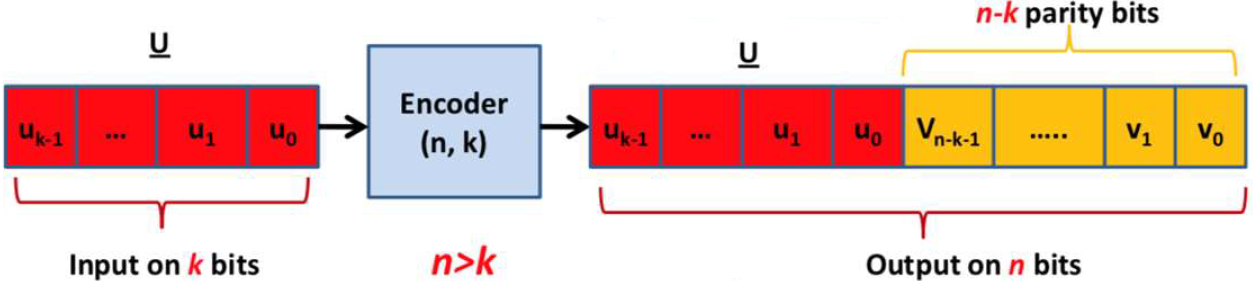
\includegraphics[width=\linewidth]{images/linear_block_codes.png}
\end{figure}
Si le mot à coder est $\overrightarrow{x}$ :

\underline{Encoder}: $G_s = (I_{k\times k}|P_{k\times n-k})$.

\underline{Decoder}: $H_s = (P_{n-k\times k}^T|I_{n-k\times n-k})$.

\underline{Code }: $\overrightarrow{y} = \overrightarrow{x}G_s$.

\underline{Erreur pendant la transmission}: $\overrightarrow{y_e}=\overrightarrow{y}+\overrightarrow{e}$.

\underline{Syndrome}: $\overrightarrow{s}= \overrightarrow{y}H_s^T+\overrightarrow{e}H_s^T$.

Pour mettre une matrice sous forme systématique il faut faire une combinaison linéaire des lignes ou colonnes.

Matrice de contrôle pour un code de Hamming (7,4) :

\setlength{\abovedisplayskip}{-2pt}
\setlength{\belowdisplayskip}{-2pt}
\begin{wrapfigure}{l}{5cm}
    \begin{equation*}
        H = \begin{pmatrix}
            0 & 0 & 0 & 1 & 1 & 1 & 1 \\
            0 & 1 & 1 & 0 & 0 & 1 & 1 \\
            1 & 0 & 1 & 0 & 1 & 0 & 1
        \end{pmatrix}
    \end{equation*}
\end{wrapfigure}
Dans ce cas $H\neq H_s$ car elle n'est pas canonique symétrique.
Si $\overrightarrow{s} = 0$ alors il n'y a pas d'erreur, sinon il y a une erreur. La position de
l'erreur est donnée par le syndrome. Il faut donc soustraire le syndrome à $\overrightarrow{y}$
pour trouver le mot d'origine.

Table avec quelques codes de Hamming et rendement associé:

\begin{tabular}{|ccccccc|}
    \hline
    $n - k$ & 2     & 3     & 4     & 5     & 6     & 7     \\
    \hline
    $n$     & 3     & 7     & 15    & 31    & 63    & 127   \\
    \hline
    $k$     & 1     & 4     & 11    & 26    & 57    & 120   \\
    \hline
    $\eta$  & 0.333 & 0.571 & 0.733 & 0.839 & 0.905 & 0.945 \\
    \hline
\end{tabular}

\textbf{Cyclic code}

\underline{Un code linéaire} (n, k) est dit cyclique si tout décalage cyclique d'un mot code est encore un mot code.

\setlength{\intextsep}{-5pt}
\begin{wrapfigure}{l}{0.2\textwidth}
    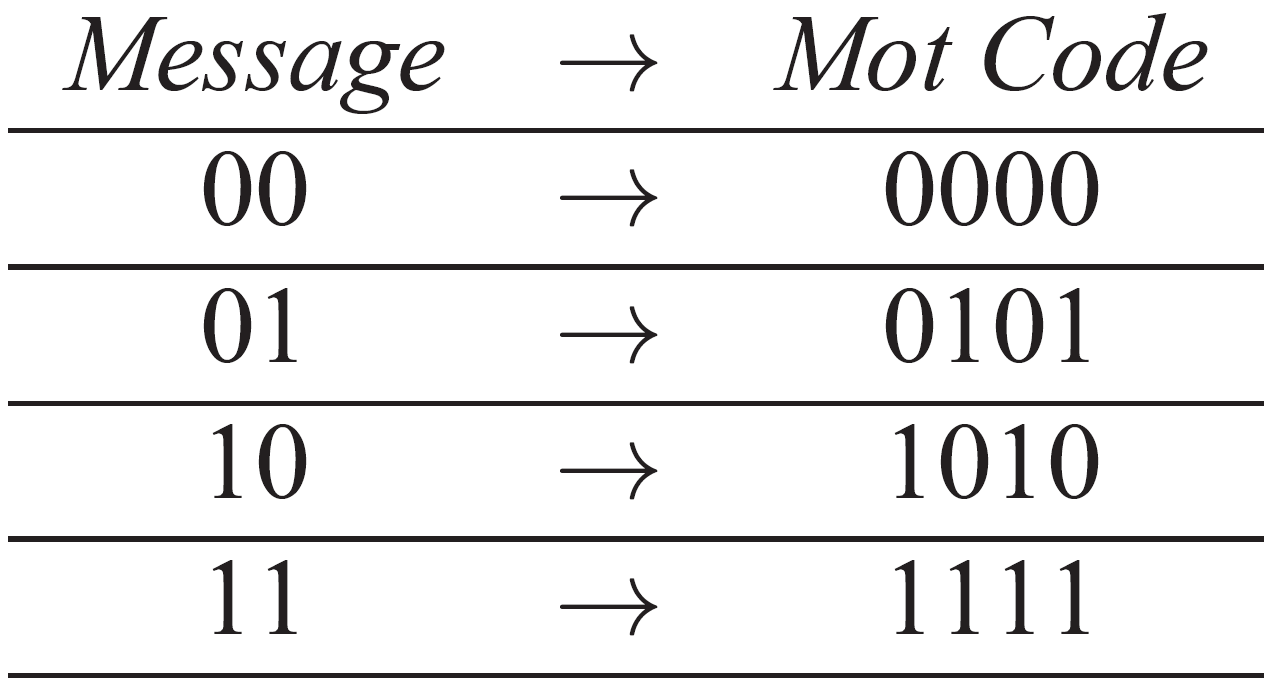
\includegraphics[width=\linewidth]{images/code_cyclique.png}
\end{wrapfigure}
\underline{Propriété 1:}

Le générateur d'un code cyclique est le code polynomial non nul de
degré minimal. Pour le cas dans le tableau: $0101$ s'écrit donc $0X^3 + 1X^2 + 0X + 1 =X^2+1$
qui est bien de degré $4-2 = 2$

\underline{Propriété 2:}

Le code polynomial non nul de degré minimal d'un code cyclique
(n, k) divise le polynôme $1 + X^n$ : $(1 + X^2)(1 + X^2) = 1 + 2X^2 + X^4 = 1 + X^4 + (1 + 1)X^2 = 1 + X^4$
(addition binaire donc $1+1=0$)

\columnbreak

\underline{Propriété 3:}

Afin d'engendrer le code on multiplie les polynômes correspondant
aux messages d'information par le polynôme générateur.

\setlength{\intextsep}{-2pt}
\begin{figure}[H]
    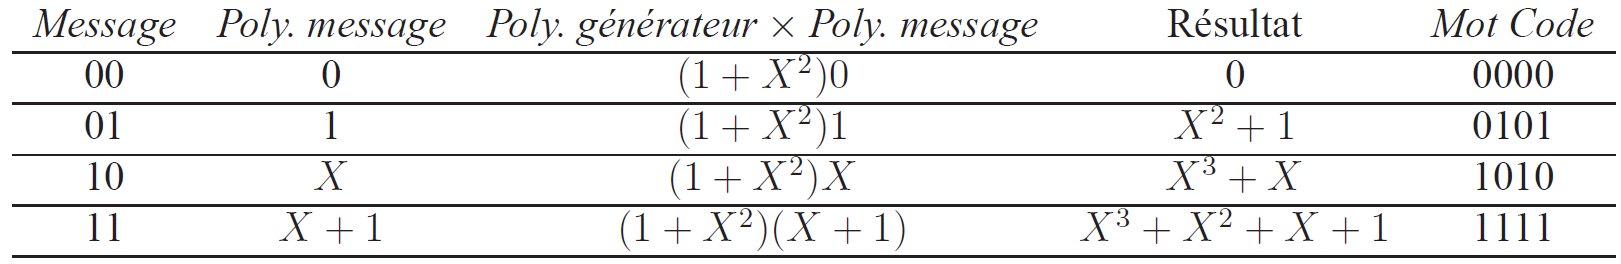
\includegraphics[width=\linewidth]{images/generer_code_cyclique.png}
\end{figure}

\underline{Propriété 4:}

Les k décalages cycliques du mot code correspondant au polynôme
non nul de degré minimal forment une base du code :
$0000 = 0 \times 1010 = 0 \times 0101$, $1010 = 1 \times 1010$, $0101 = 1 \times 0101$ et
$1111 = 1 \times 0101 + 1 \times 1010$

\textbf{Encodage systématique:} (n, k)

$G_s = (I_{k\times k}|P_{k\times n-k})$.
L'encodage systématique permet de retrouver le message d'origine en ne prenant que les
$k$ premiers bits du mot code, les $n-k$ derniers bits sont les bits de parité.

\underline{Multiplier le message:} $i(X)\rightarrow X^{n-k}i(X)$.

\underline{Diviser par le polynôme générateur}: $X^{n-k}i(X)=a(X)g(X)+r(X)$

\underline{Ajouter le reste à la fin du message} compte tenu de l'addition binaire:

$X^{n-k}i(X)+r(X)=a(X)g(X)$

\underline{Exemple}:

Trouver pour un code cyclique (7, 4) l’encodage systématique de $1010$.

Trouver le générateur: $1+X^7=(1+X)(1+X+X^3)(1+X^2+X^3)$, on prend $g(X)=1+X+X^3$.

Calculer: $X^{n-k}i(X)=X^3(X^3+X)=X^6+X^4$.

\setlength{\abovedisplayskip}{-2pt}
\setlength{\belowdisplayskip}{-2pt}
\begin{wrapfigure}{l}{6cm}
    \[
        \begin{array}{r|r}
            X^6 + X^4\phantom{{}+6} & X^3 + X + 1 \\ \cline{2-2}
            + X^6 + X^4 +X^3        & X^3 + 1     \\ \cline{1-1} \\[\dimexpr-\normalbaselineskip+\jot]
            X^3\phantom{{}+6}                     \\
            +X^3 + X + 1                          \\ \cline{1-1} \\[\dimexpr-\normalbaselineskip+\jot]
            X + 1
        \end{array}
    \]
\end{wrapfigure}
Diviser par $g(X)$: $X^6+X^4=(X^3 + X + 1)(X^3 + 1)+X+1$

Ajouter le reste au calcul: $X^6+X^4+X+1\rightarrow 1010011$

Schéma équivalent au circuit de division $\frac{u(X)}{g(X)}$
\vspace*{0.5cm}
\begin{figure}[H]
    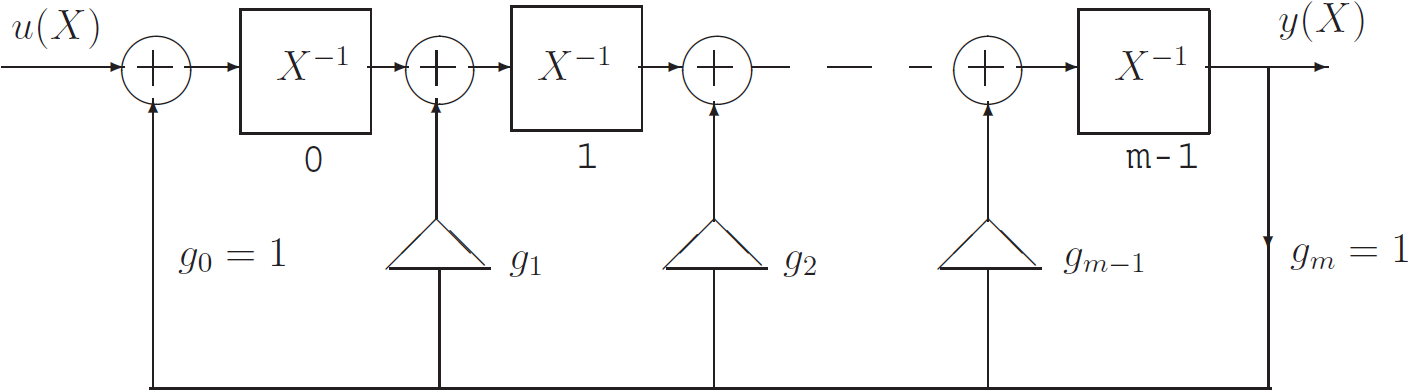
\includegraphics[width=\linewidth]{images/schema_division.png}
\end{figure}

\columnbreak

\underline{Décodage:}

On divise le block reçu par $g(x)$, si le reste est nulle le
résultat est juste autrement il est faux. Le syndrome est
le reste de la division par $g(x)$.

On calcule un code à partir du message reçu puis on
compare ce code avec celui qui est reçu. Ceci ne marche
que pour les codes systématiques.

\textbf{BCH code:}

Les codes BCH sont construits pour corriger t erreurs. Pour
tout couple d'entiers positifs $m$ $(m \geq 3)$ et $t$ $(t < 2m-1)$ on peut
montrer qu'il existe un code binaire BCH avec les
paramètres suivants :

\underline{Number of parity check-symbols}: $n-k\leq mt$.

J'ai rien compris ça à l'air trop compliqué.

\textbf{Convolutional code:}

Les codeurs convolutifs ont une mémoire qui influe sur les $n$ bits de sortie à partir des $k$
bits d'entrée et des $m$ états internes.

\underline{Taux de codage}: $R=\frac{1}{n}$

\underline{Code state}: le contenu de la mémoire, il y a $2^{mk}$ états différents.

\underline{Exemple de diagramme}: $n=2$, $k=1$, $m=3$ (2,1,3)

\begin{figure}[H]
    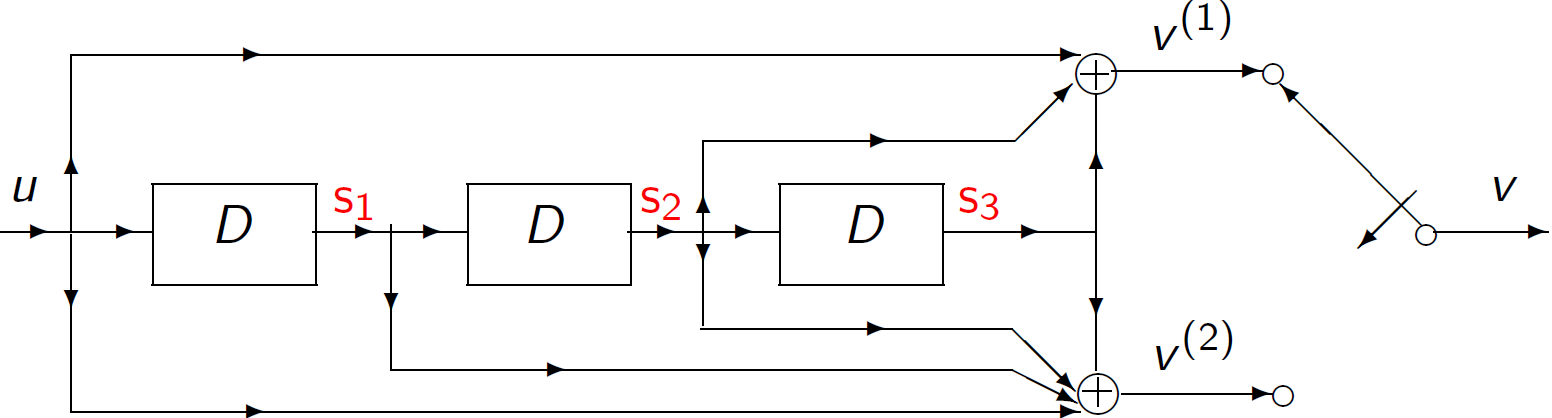
\includegraphics[width=\linewidth]{images/conv_coding_diagramme.png}
\end{figure}

Pour chaque état on peut trouver on trouve la dépendance temporelle :
$s_1=u(n-1)$,

$s_2=s_1(n-1)$,

$s_3=s_2(n-1)$

Pour chaque output écrire leur dépendance :

$v^{(1)}=u(n)+s_2(n)+s_3(n)$,

$v^{(2)}=u(n)+s_1(n)+s_2(n)+s_3(n)$

En transformée de Z cela donne:

$V^{(1)}(z)=(1+z^{-2}+z^{-3})U(z)$,

$V^{(2)}(z)=(1+z^{-1}+z^{-2}+z^{-3})U(z)$

Les polynômes générateurs sont:

$g^{(1)}=(1,0,1,1)$,

$g^{(2)}=(1,1,1,1)$.

$V^{(1)}$ est donc la convolution entre $u(n)$ et $g^{(1)}$.

\columnbreak
\underline{Exemple complet}:
\begin{figure}[H]
    \begin{minipage}{0.255\textwidth}
        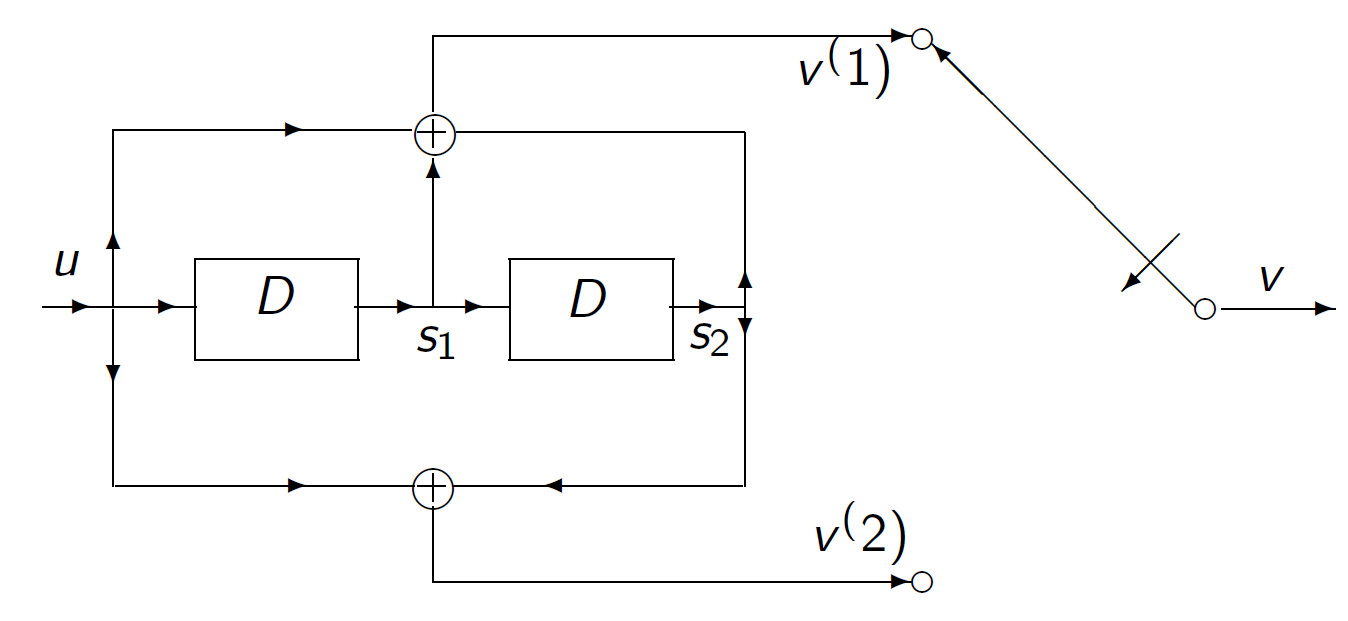
\includegraphics[width=\linewidth]{images/conv_coding_diagramme_2.png}
    \end{minipage}%
    \begin{minipage}{0.255\textwidth}
        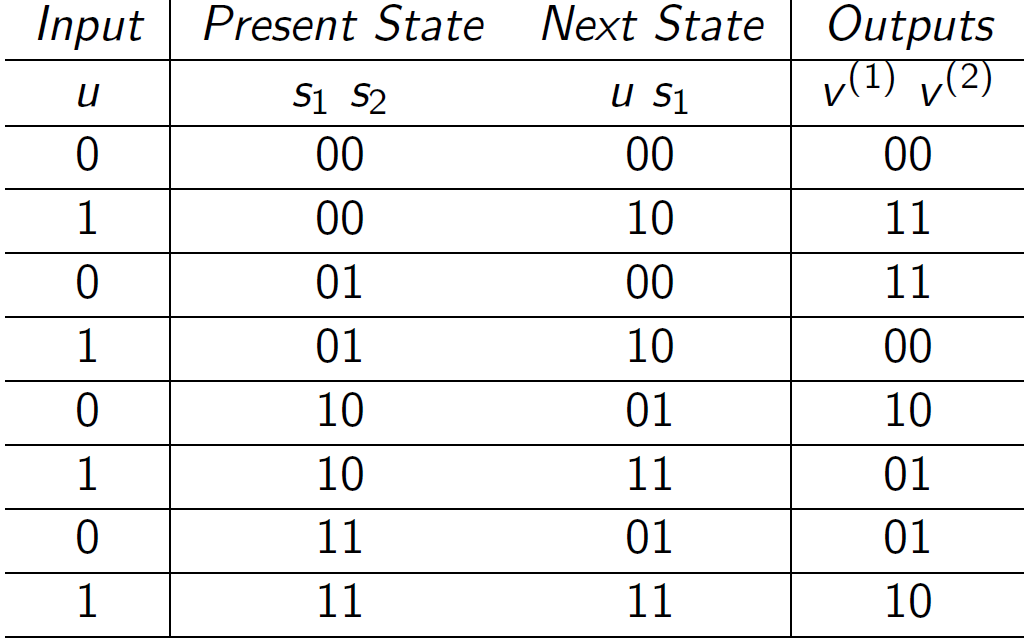
\includegraphics[width=\linewidth]{images/conv_coding_table_2.png}
    \end{minipage}
\end{figure}
L'\underline{encoder state diagram} (droite): représente les états du codeur et les transitions entre
les états.

En rouge \textcolor{red}{les états}, en bleu \textcolor{blue}{les inputs} (nouvelles
valeurs de $u(n)$) et en vert \textcolor{green}{les outputs} (valeurs de $v(n)$).

De Cela on peut construire le \underline{diagramme de treillis} (gauche) qui représente les chemins
possibles dans le codeur.
\begin{figure}[H]
    \begin{minipage}{0.15\textwidth}
        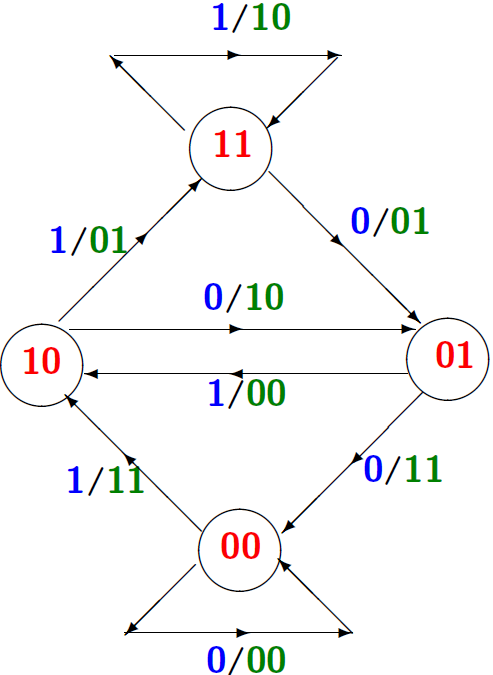
\includegraphics[width=\linewidth]{images/conv_coding_encoder_state_diagram_2.png}
    \end{minipage}%
    \begin{minipage}{0.35\textwidth}
        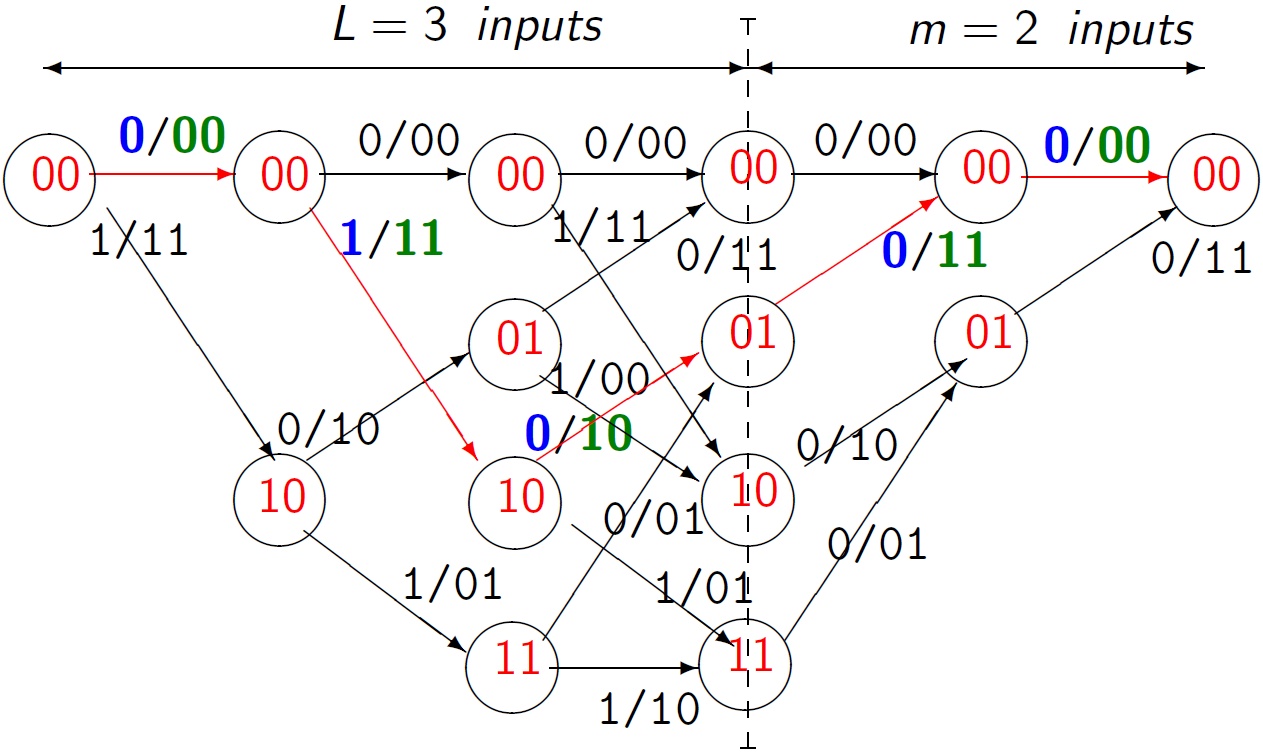
\includegraphics[width=\linewidth]{images/conv_coding_treillis_diagram_2.png}
    \end{minipage}
\end{figure}
Ce diagramme de treillis représente la réponse à une entrée \textcolor{blue}{$u(n)=010$} qui donne en sortie
\textcolor{green}{$v(n)=0011101100$}.

Le décodeur d'un code convolutif cherche le chemin dans le treillis qui correspond le
mieux aux données reçues (l'observation) on utilise \underline{l'algorithme de Viterbi} pour cela.
Le best fit peut se calculer de deux manières différentes:

Par la distance de Hamming entre les bits reçus et attendus.

Par la distance euclidienne au carré entre les valeurs reçues et attendues.
\begin{figure}[H]
    \begin{minipage}{0.24\textwidth}
        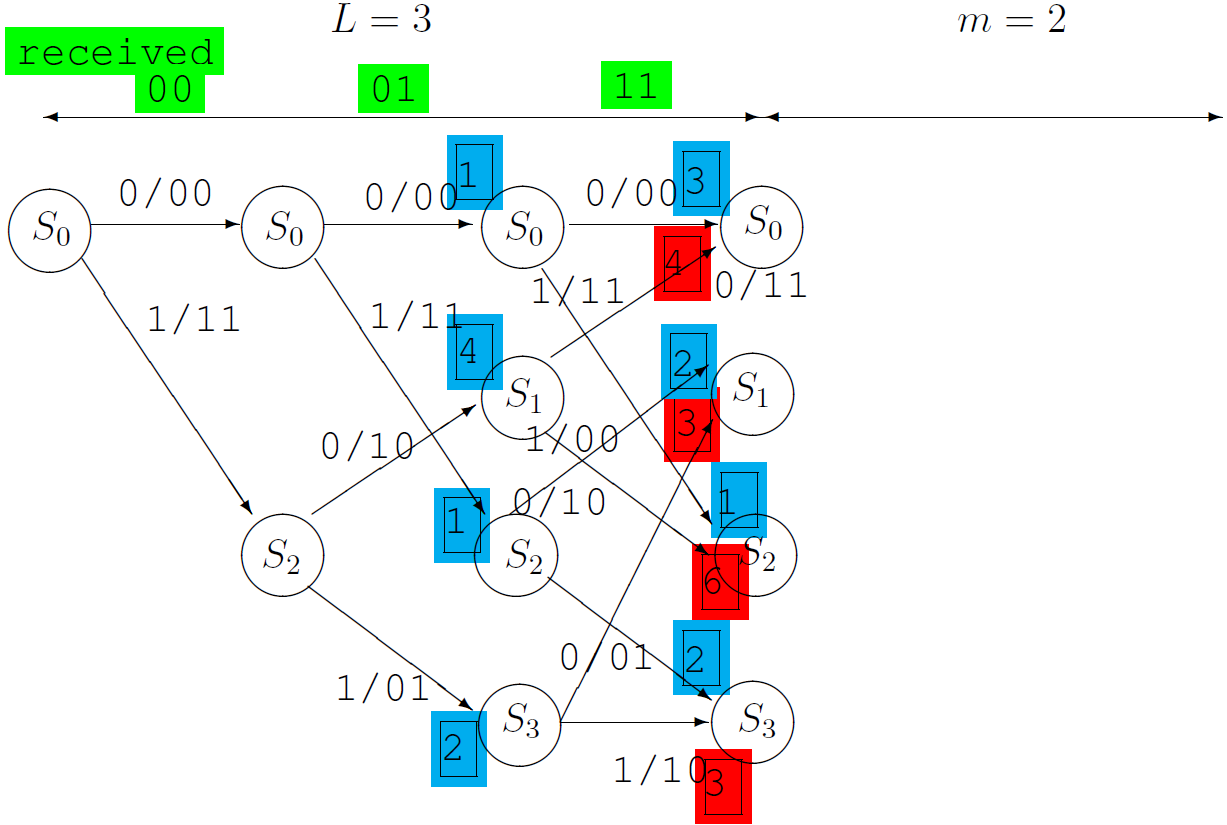
\includegraphics[width=\linewidth]{images/conv_coding_viterbi_1.png}
    \end{minipage}
    \begin{minipage}{0.24\textwidth}
        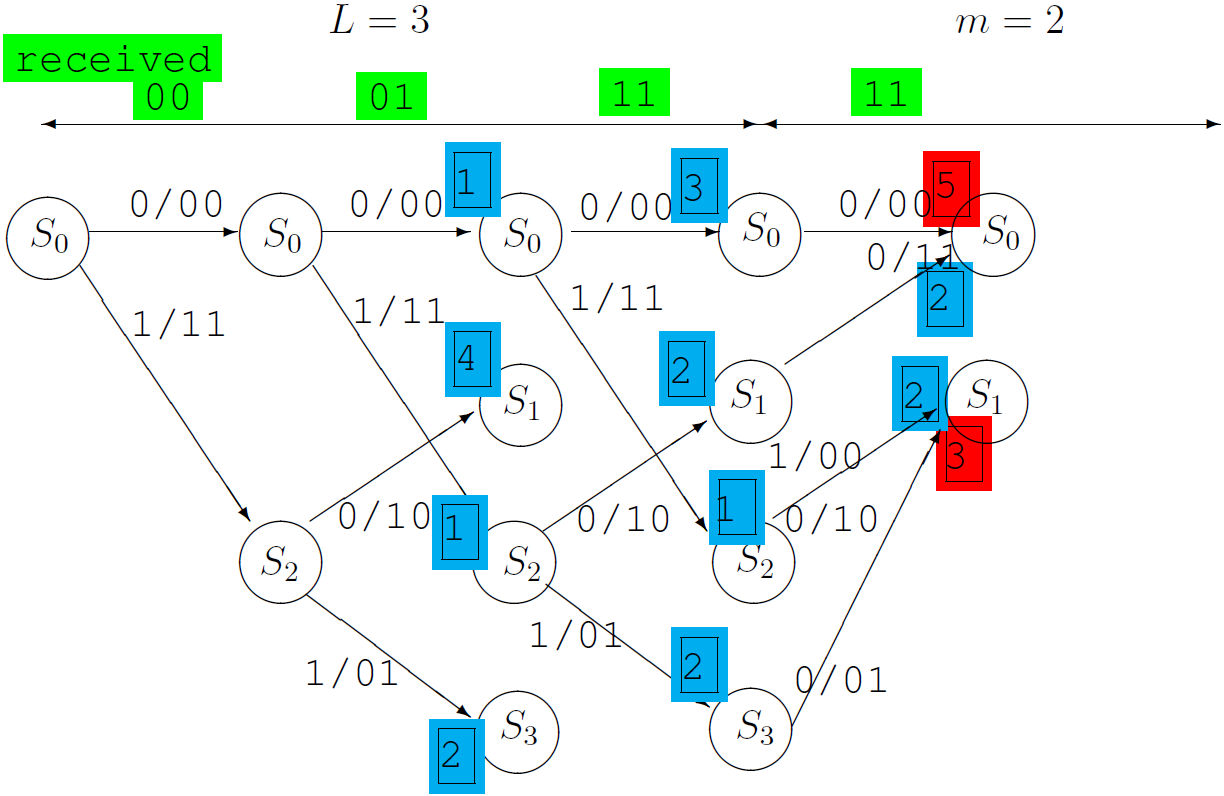
\includegraphics[width=\linewidth]{images/conv_coding_viterbi_2.png}
    \end{minipage}
\end{figure}
\needspace{5\baselineskip}
\begin{wrapfigure}{l}{0.24\textwidth}
    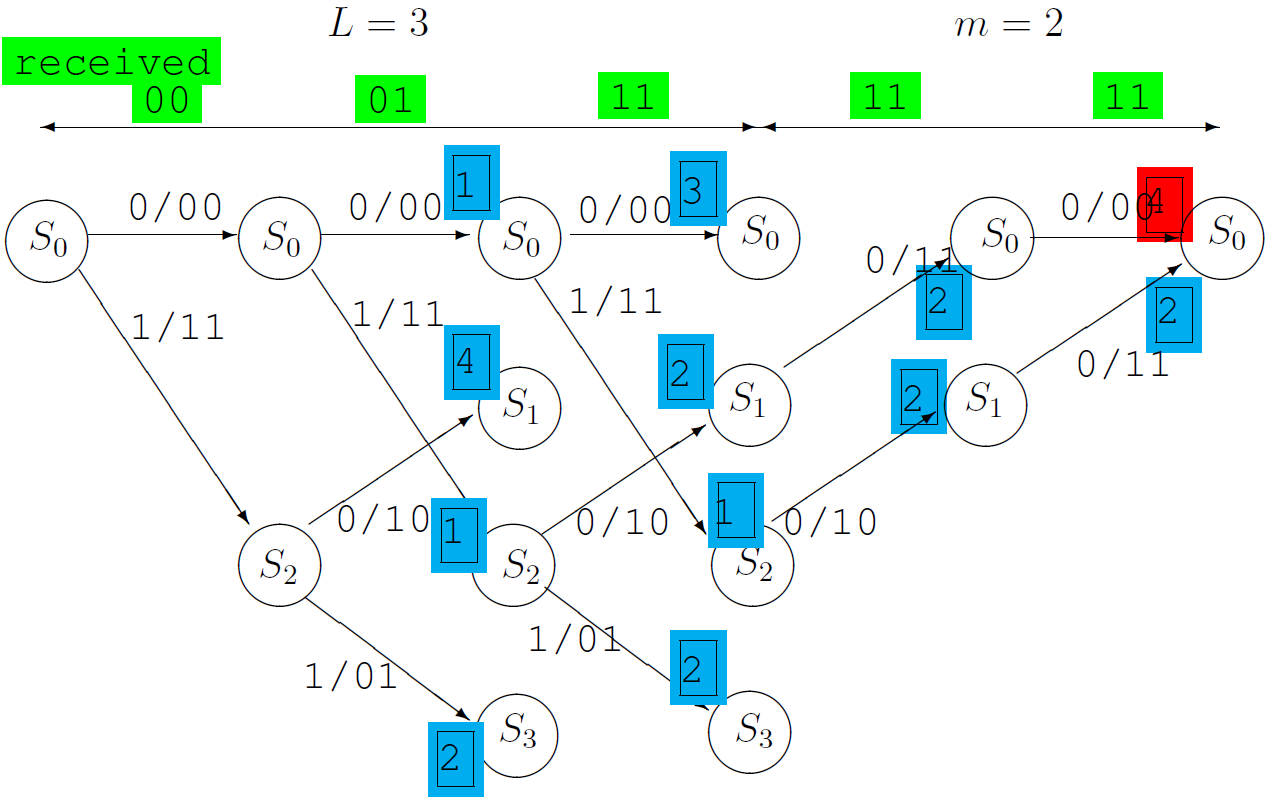
\includegraphics[width=0.24\textwidth]{images/conv_coding_viterbi_3.png}
\end{wrapfigure}
Le message transmis est : $00 01 11 11 11$ en utilisant la distance de Hamming comme metric pour
le best fit. Dans ce cas on trouve un chemin avec un distance de Hamming de 2. Le message corrigé est
$00 00 11 10 11$ la séquence d'entrée détectée est $001$.\\







    \subsection*{Wireless Channel}
Le but est de définir le canal sans fil avec plus de précision que le modèle AWGN et de donner un
plan de référence plus réaliste pour les systèmes de communication.

\textbf{Fading lent:}

sont des modèles basés sur la puissance du signal en fonction
de la distance.

\underline{Open sky attenuation}

Friis: $P_r=P_t G_r G_t\left(\frac{\lambda}{4\pi d}\right)^2[W]$ avec $\lambda=\frac{C}{f}[m]$

Atténuation: $Att=\left(\frac{4\pi d}{\lambda}\right)^2$ Il faut prendre la vitesse de la lumière à $C=300 000$

Friis en dB: $P_r|_{dBm}=P_t|_{dBm}+G_r|_{dBi}+G_t|_{dBi}+20\log_{10}(\lambda)-20\log_{10}(4\pi d)$
Pour une antenne omnidirectionnelle $G_r|_{dBi}=G_t|_{dBi}=0$

Friis avec obstacle: $P_r=P_t G_r G_t\frac{\lambda^2}{(4\pi)^2 d\gamma}$
avec $\gamma$ le coefficient de propagation qui dépend de l'environnement:

\begin{tabular}{l|l}
    Environment                        & $\gamma$   \\ \hline
    Free space:                        & 2          \\
    Urban area cellular radio:         & 2.7 to 3.5 \\
    Shadowed urban cellular radio:     & 3 to 5     \\
    Inside a building - line of sight: & 1.6 to 1.8 \\
    Obstructed in building:            & 4 to 6     \\
    Obstructed in factory:             & 2 to 3
\end{tabular}

\underline{Shannon with fading}:

La capacité du canal: $C_{fading}=B\log_2(1+\frac{S}{N}|h|^2)$ avec $h$ le fading un nombre complexe

Comme $h$ est une variable aléatoire, on utilise la moyenne statistique:
$C_{fading}=E[B\log_2(1+\frac{S}{N}|h|^2)]$

\underline{Log-distance model}: $P_r=P_t\cdot\text{Att}_{d_0}(\frac{d_0}{d})^\gamma X_g$
C'est une amélioration du modèle de Friis qui prend en l'aléatoire du canal. Basé sur une atténuation
à $d_0$ et un coefficient $\gamma$ qui dépend de l'environnement. $X_g$ variable aléatoire qui
qui correspond au fading.

\underline{Ground reflection model}:

\begin{figure}[H]
    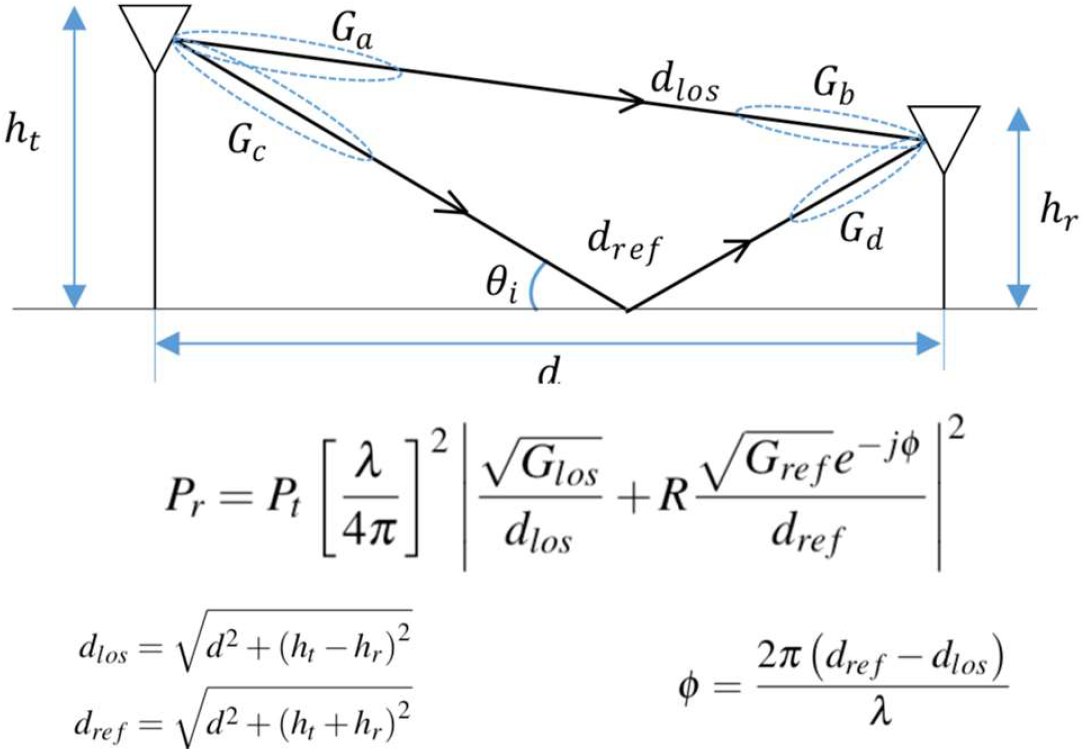
\includegraphics[width=\linewidth]{images/ground_reflection_model.png}
\end{figure}

\underline{Fresnel zone}: $R=\frac{1}{2}\sqrt{\frac{cD}{f}}$ avec D la distance entre les antennes.
C'est une sorte de globe elliptique qui entoure la ligne de visée.

\textbf{Fading rapide:}

sont des modèles basés sur la distribution statistique de l'amplitude
du signal en fonction des réflexions multiples.

\underline{Rayleigh distribution}: $p(x)=\frac{x}{\sigma^2}e^{-\frac{x^2}{2\sigma^2}}$ avec $x$
l'amplitude du signal et $\sigma$ l'écart type.

\underline{Rice distribution}: $p(x)=\frac{x}{\sigma^2}e^{-\frac{x^2+k^2}{2\sigma^2}}I_0\left(\frac{kx}{\sigma^2}\right)$
avec $k$ le facteur de K et $I_0$ la fonction de Bessel modifiée d'ordre 0.

\underline{Nakagami distribution}: $p(x)=\frac{2m^m}{\Gamma(m)\Omega^m}x^{2m-1}e^{-\frac{m}{\Omega}x^2}$
avec $m$ le facteur de Nakagami et $\Omega$ le facteur de fading.


\end{multicols*}
\subsection*{Modulation}
\begin{multicols*}{4}
    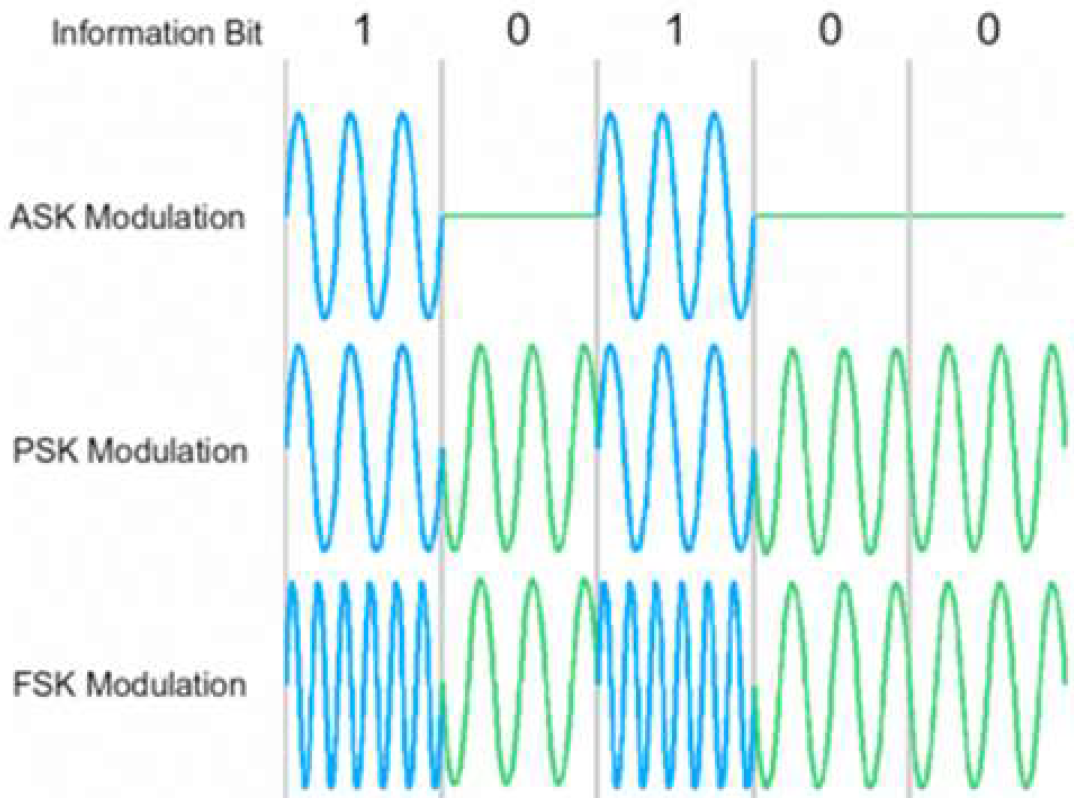
\includegraphics[width=\columnwidth]{images/binary_modulation.png}
    AM: ASK (Amplitude Shift
    Keying)

    PM: PSK (Phase Shift
    Keying) comme on utilise la phase du signal, les nombres complexes sont utilisés.

    FM: FSK (Frequency Shift Keying)

    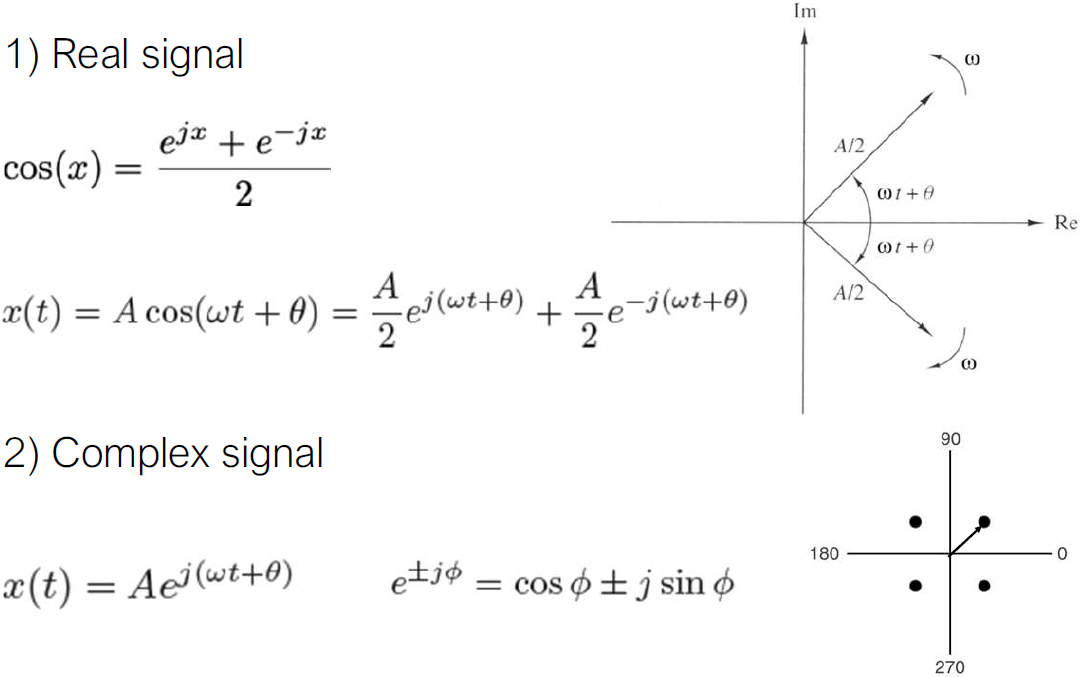
\includegraphics[width=\columnwidth]{images/nombres_complexes.png}
    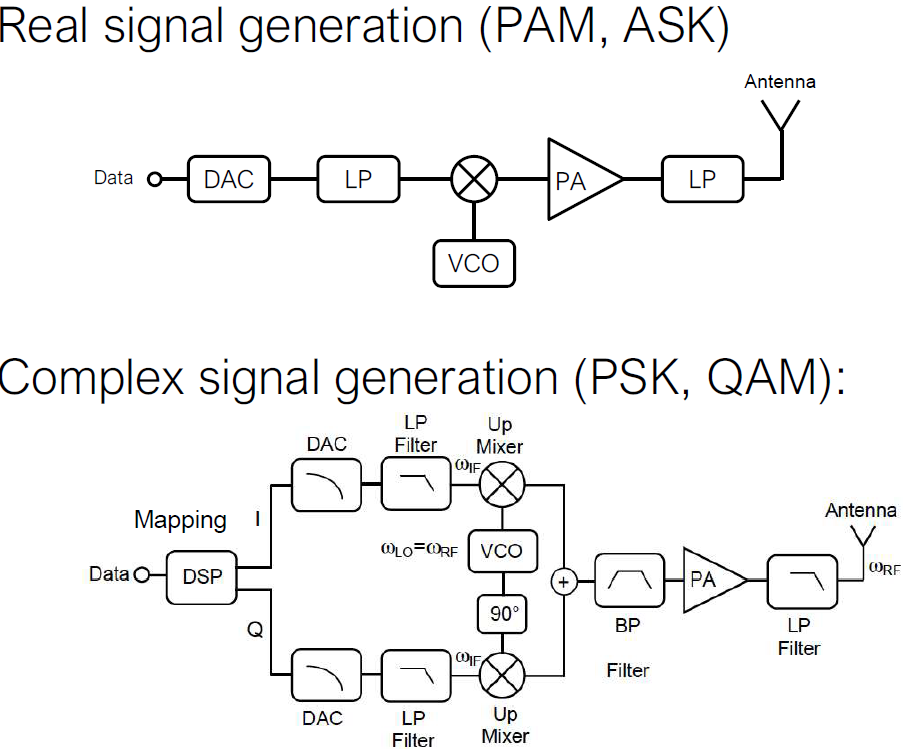
\includegraphics[width=\columnwidth]{images/signal_generation.png}
    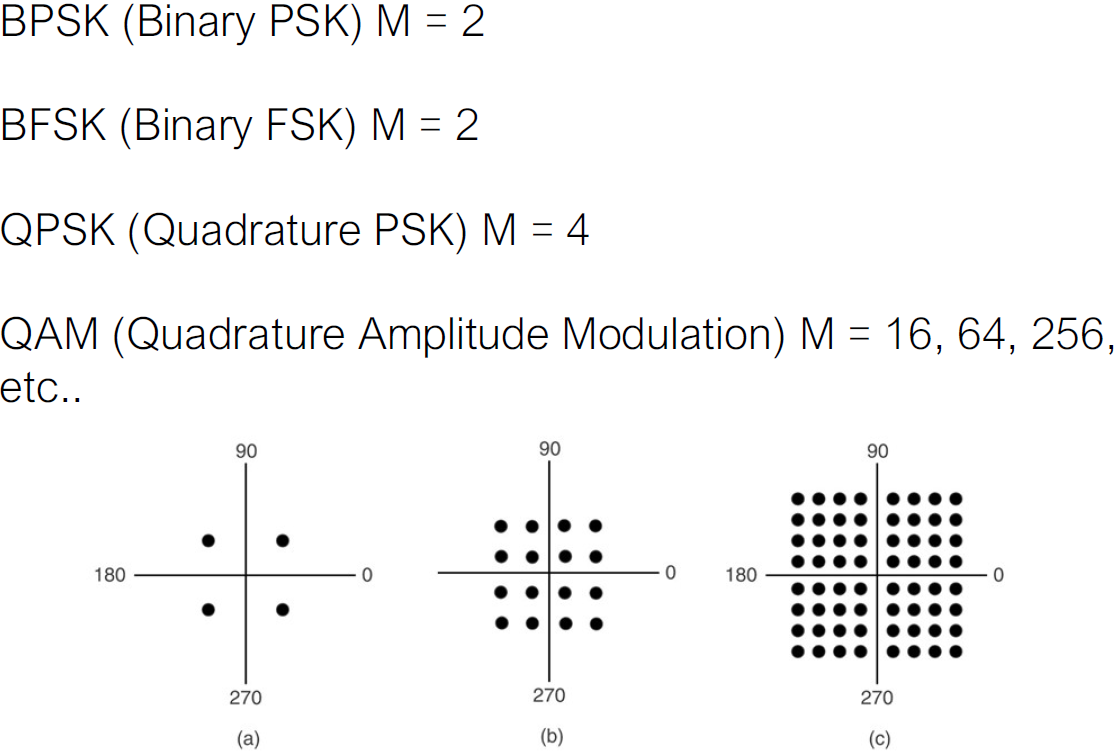
\includegraphics[width=\columnwidth]{images/bfsk_qpsk.png}
    Chaques symboles est représenté par un vecteur dans le plan complexe. La phase du vecteur
    représente le symbole et la norme du vecteur représente l'amplitude du signal.

    Bit energy to noise ratio: Bit energy over noise
    spectral density required for demodulation. It is
    commonly called $E_b/N_0$

    Symbol energy to noise ratio: Symbol energy over
    noise spectral density required for demodulation. It is
    commonly called $E_s/N_0$

    Signal to noise ration : $SNR = \frac{S}{N}=\frac{E_sR}{N_0B}$ where $R_b$ is the bit rate.

    Relation : $\frac{E_s}{N_0}=\frac{E_b}{N_0}\log_2M$

    BER : $\frac{\text{Error count}}{\text{total transmitted bits}}$

    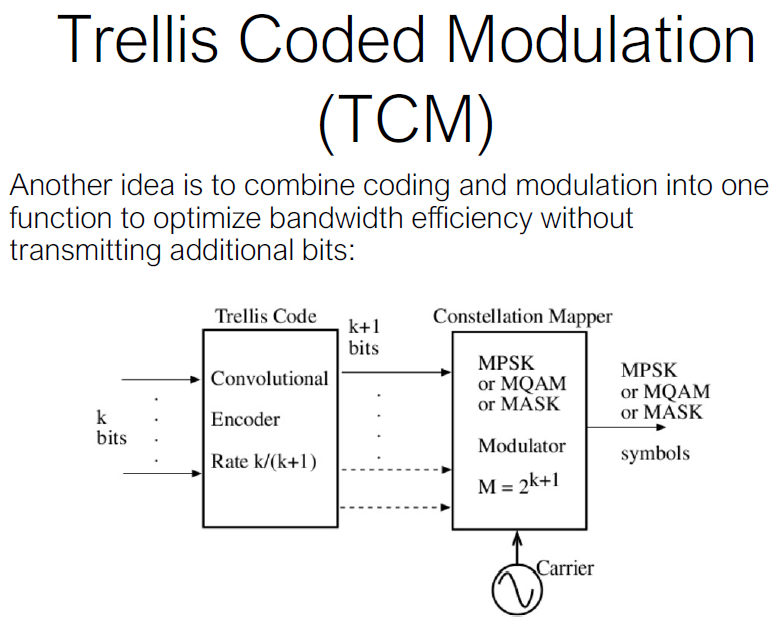
\includegraphics[width=\columnwidth]{images/merde1.png}
    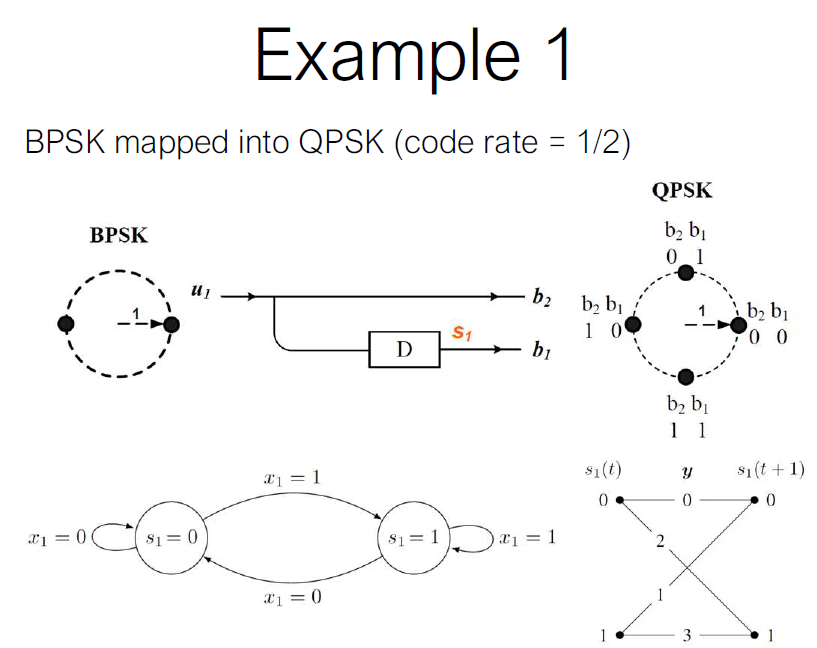
\includegraphics[width=\columnwidth]{images/merde2.png}
    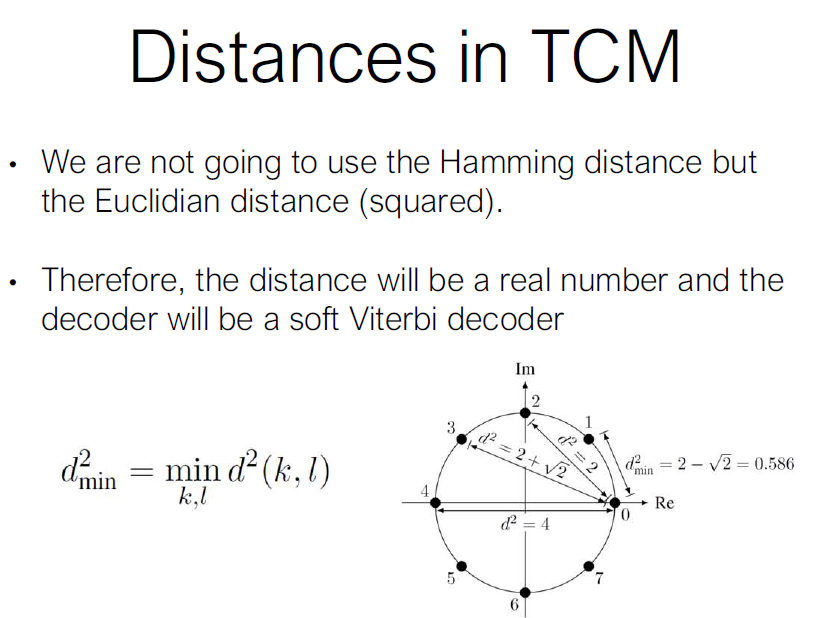
\includegraphics[width=\columnwidth]{images/merde3.png}
    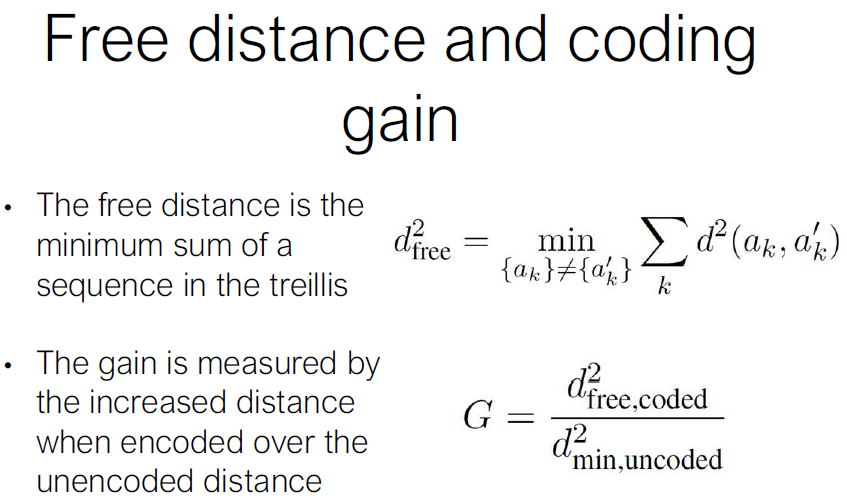
\includegraphics[width=\columnwidth]{images/merde4.png}
    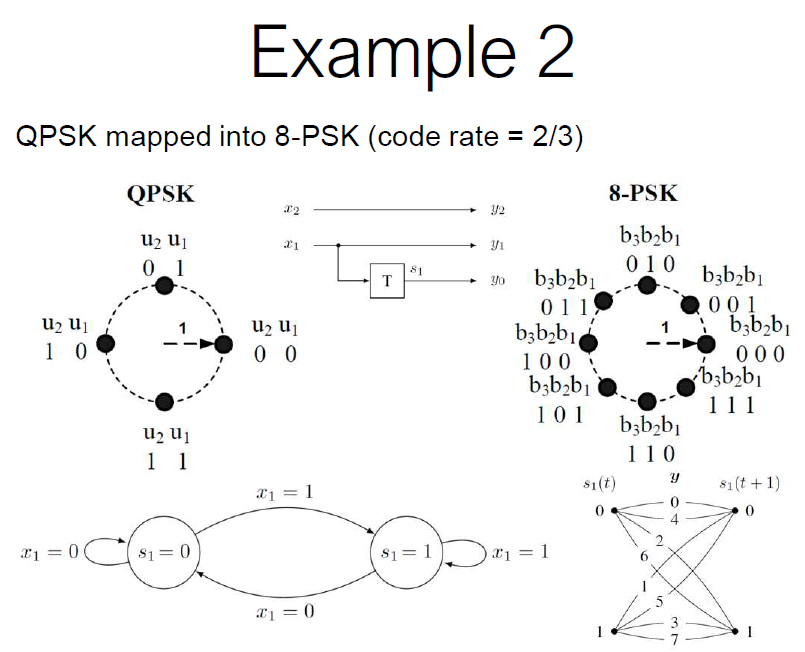
\includegraphics[width=\columnwidth]{images/merde5.png}
    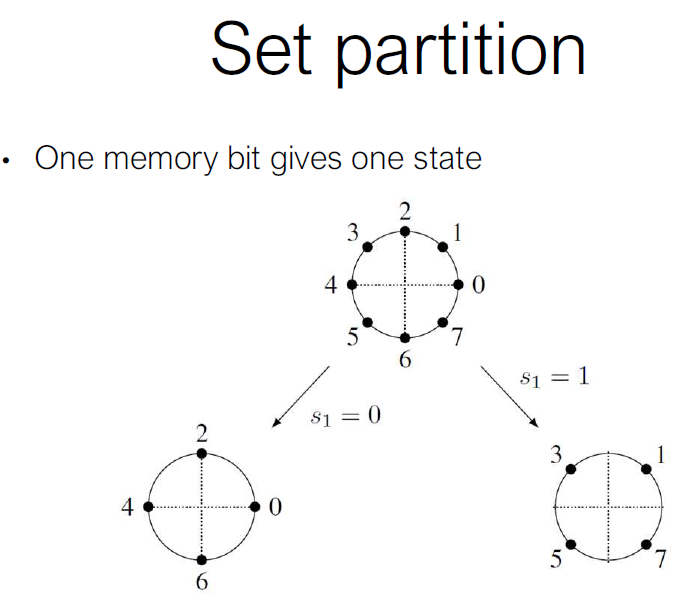
\includegraphics[width=\columnwidth]{images/merde6.png}
    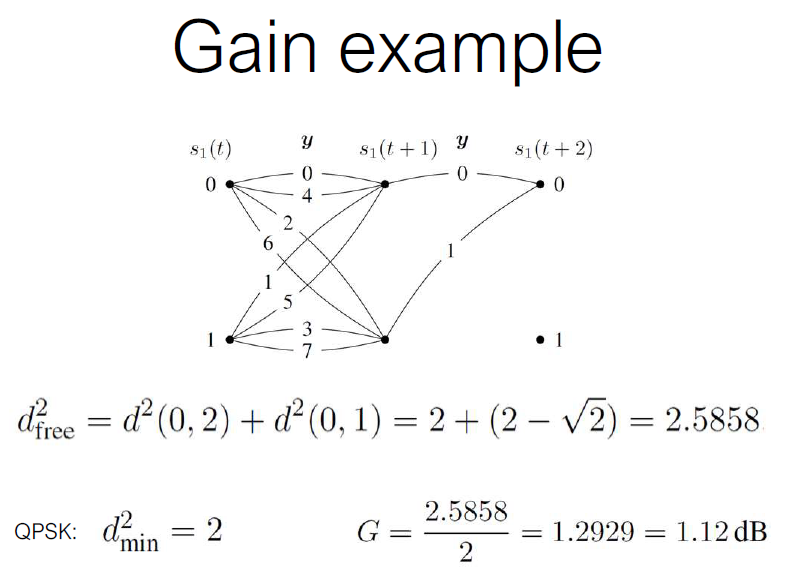
\includegraphics[width=\columnwidth]{images/merde7.png}
    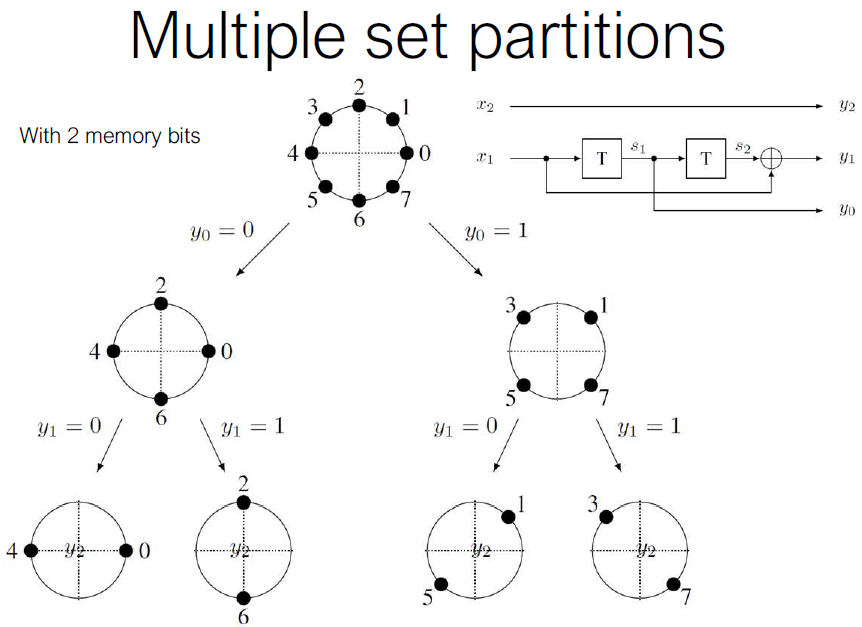
\includegraphics[width=\columnwidth]{images/merde8.png}
    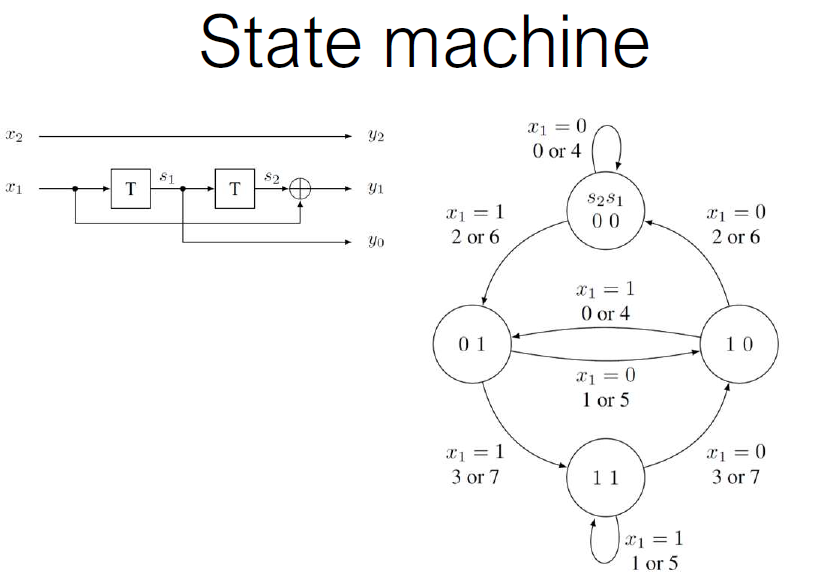
\includegraphics[width=\columnwidth]{images/merde9.png}
    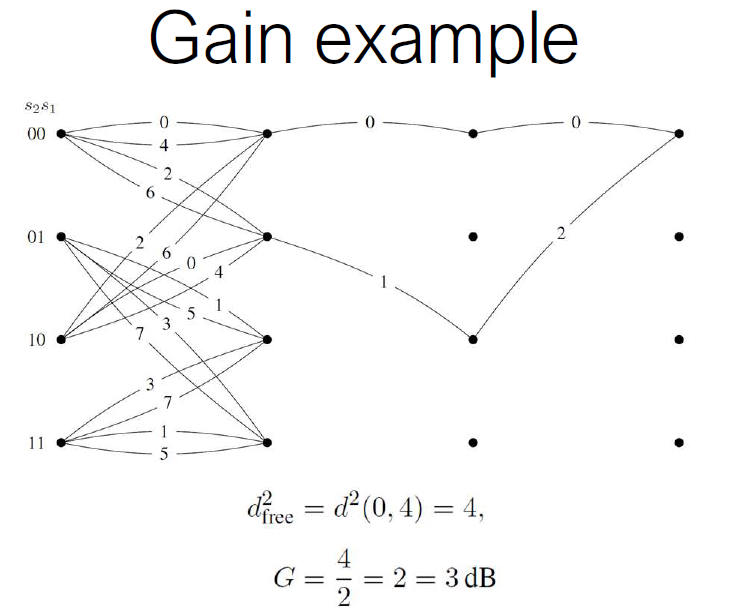
\includegraphics[width=\columnwidth]{images/merde10.png}
\end{multicols*}


\begin{multicols*}{2}
    \subsection*{Multiple Access}
\textbf{Time Division Duplex TDD:}

The duplexer is a switch allowing to
separate transmit (Tx) and receive (Rx).It is placed between the antenna and
amplifiers. It is simple but only allows a half-duplex communication.

\textbf{Frequency Division Duplex FDD:}

A diplexer is a dual filter that split Tx and Rx in two
frequency channels. We can compare it to frequency multiplexer. It allows full duplex transmission.

\textbf{Carrier Sense Multiple Access CSMA:}

The idea is to listen to the channel before transmitting.
The disadvantage of this system is the potential collision occurring when two transmitters
start to emit at the same time.

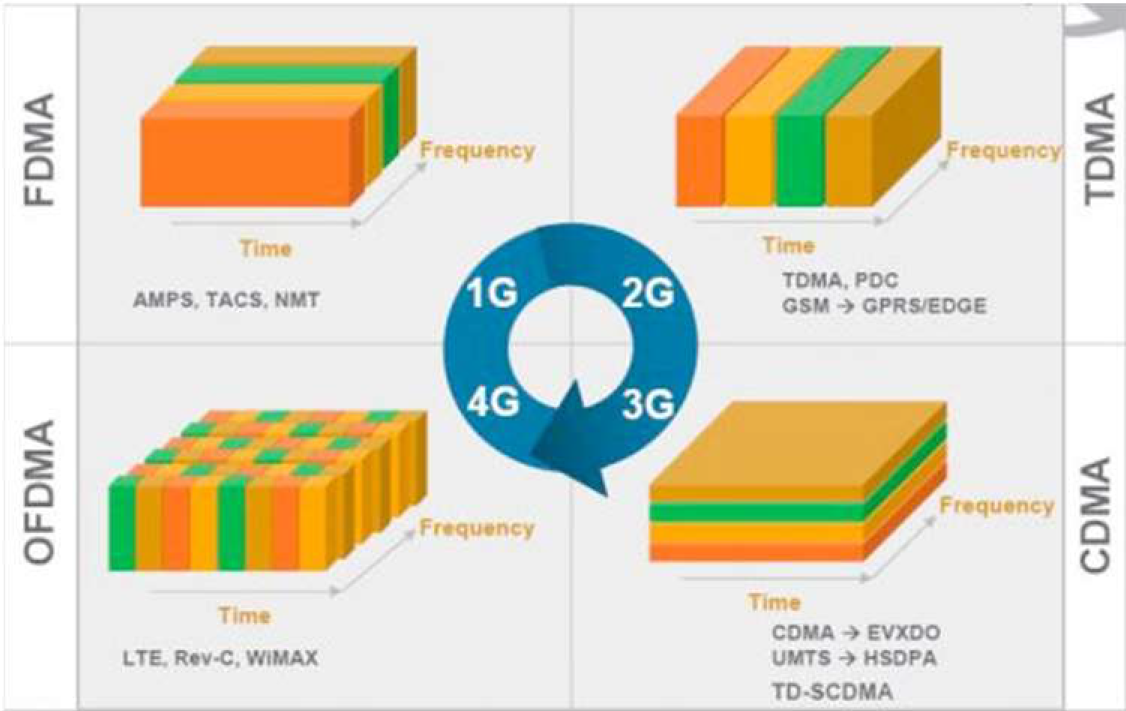
\includegraphics[width=\columnwidth]{images/multiple_access_comparison.png}

% \setlength{\intextsep}{-5pt}
% \begin{wrapfigure}{r}{0.3\textwidth}
%     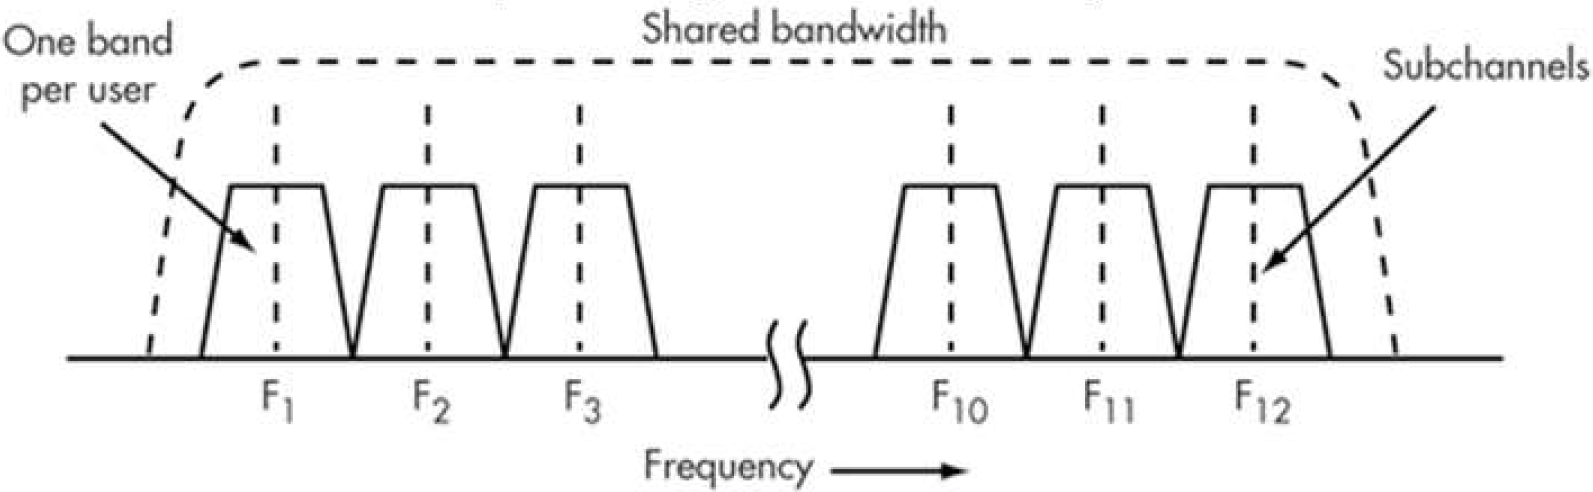
\includegraphics[width=\linewidth]{images/fdma.png}
% \end{wrapfigure}
\textbf{Frequency Division Multiple Access FDMA:}

Used in 1G. Allocation of
one frequency channel per user. Drawbacks: Number of users limited by the available bandwidth.
If one user is alone, he cannot use all the bandwidth available.

% \needspace{5\baselineskip}
% \begin{wrapfigure}{r}{0.2\textwidth}
%     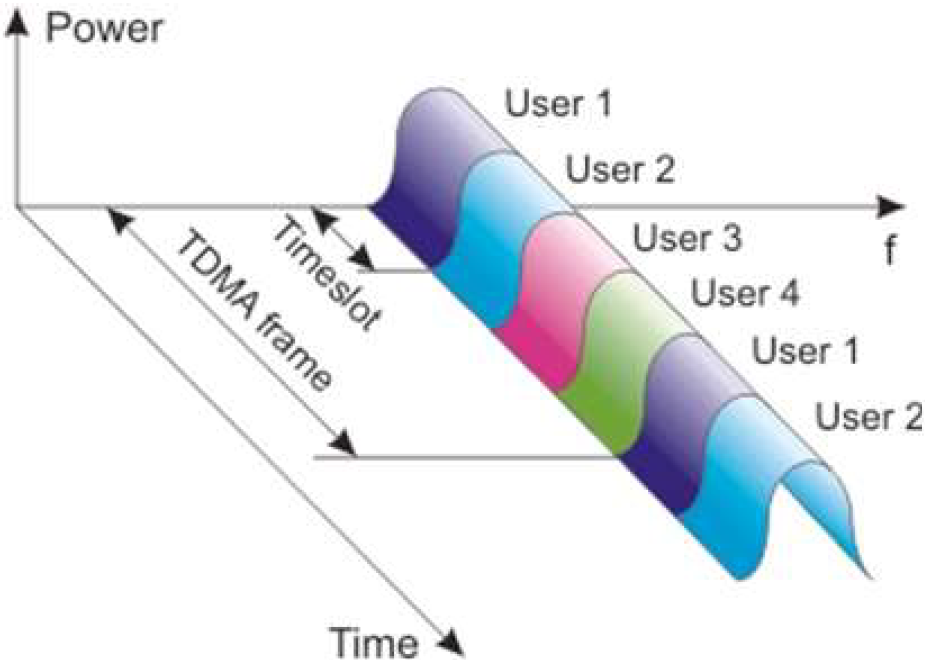
\includegraphics[width=\linewidth]{images/tdma.png}
% \end{wrapfigure}
\textbf{Time Division Multiple Access TDMA:}

Used in 2G. Allocation of one time slot per user.
Drawbacks: Time sensitive. Accurate synchronization is required to avoid overlap.\\

% \needspace{5\baselineskip}
% \begin{wrapfigure}{r}{0.3\textwidth}
%     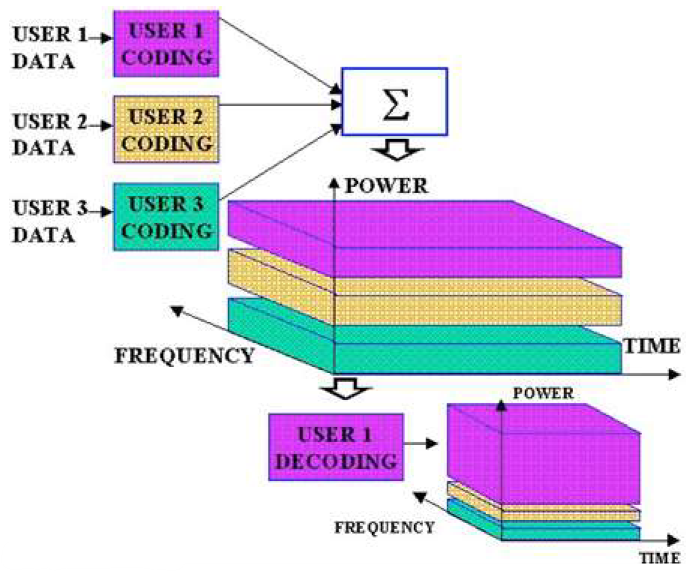
\includegraphics[width=\linewidth]{images/cdma.png}
% \end{wrapfigure}
\textbf{Code Division Multiple Access CDMA:}

Used in 3G. Each user is allocated one orthogonal
code Advantages: No spaces between channels. Simpler hardware. Robust to interferences.
Disadvantages: require power control for each user.

It uses Walsh-Hadamard orthogonal codes that have zero cross-correlation, meaning that
they do not interfere with each other when transmitted on the same channel.

Principle : Each user is allocated a Walsh-Hadamard code. At Tx, information is multiplied
by the code, this enlarge the spectrum and reduces amplitude. At Rx, we correlate the message
with the user code. Other users being orthogonal they do not interfere.

\textbf{Orthogonal Frequency Division Multiple access OFDMA:}

Used in wifi 6, 4G, 5G.
Based on OFDM (Orthogonal Frequency Division Multiplexing) a technique using FFT to create
orthogonal frequency channels.

\textbf{Space Division Multiple Access SDMA:}

Used in 5G. A cellular
system is a kind of SDMA. We divide an area in smaller zones. Advantage: more capacity and
more users. Disadvantages: Co-channel interference (between cells). Handoff (passage form one cell to another).

\textbf{SISO:}

SISO is the base system. At Rx, $x_1$ is received with fading $h_1$: $y_1=h_1x_1$

\textbf{SIMO:}

Now let us add a second antenna at Rx; we will receive 2 signals $y_1$ and $y_2$
with their associated fading $h_1$ and $h_2$: $y_1=h_1x_1$, $y_2=h_2x_1$ The capability did not
change but we can now use diversity.

\textbf{MISO:}

Let's do the same with two Tx antennas; We obtain
one equation with two unknowns $x_1$ and $x_2$. We can
not distinguish them. We need another equation (an other antenna on the receiver).
$y_1=h_1x_1+h_2x_2$, $y_2=h_1x_2^*+h_2x_1^*$

\textbf{MIMO:}

Now let's put 2 Tx antennas and 2 Rx antennas; We
get a system with two equations and 2 unknowns $x_1$
and $x_2$. We can therefore distinguish $x_1$ and $x_2$. $y_1=h_1x_1+h_2x_2$, $y_2=h_3x_1+h_4x_2$
We created a spatial multiplex and the channel capacity doubled.
MIMO is advantageous if we have enough space to put antennas. Minimum spacing is $\sfrac{\lambda}{2}$
but for full good decorrelation. 5G uses MMIMO (Massive MIMO) with 64 antennas. This allows
beaming forming (direct the beam to the user).





    \columnbreak
    \subsection*{Acquisition and Synchronization}
\textbf{Carrier Recovery:}

We want to cancel phase error. This in turn cancel
the frequency error as frequency is phase speed. We use a PLL (Phase Locked Loop)
to do so. The PLL is a feedback loop that compares the phase of the received signal
with the phase of the local oscillator. The phase error is then used to correct
the local oscillator phase.

\setlength{\intextsep}{-10pt}
\begin{wrapfigure}{r}{0.3\columnwidth}
    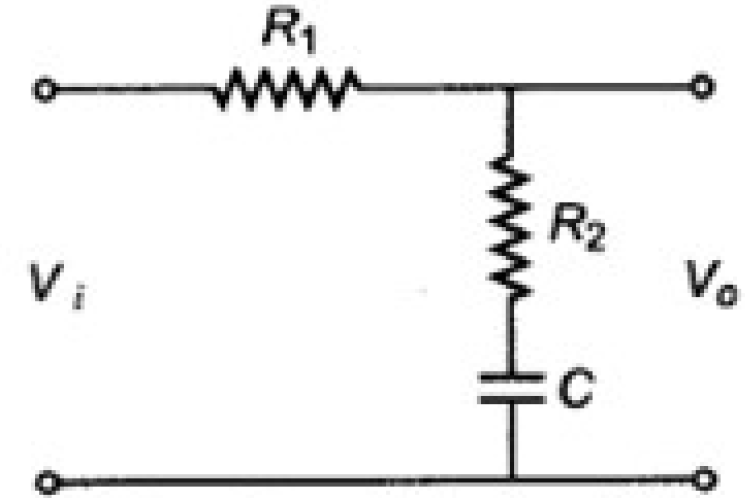
\includegraphics[width=\linewidth]{images/pll_loop_filter.png}
\end{wrapfigure}
\underline{Transfert function of the PLL:}

$H(s)=\frac{\frac{KG(s)}{s}}{1+\frac{KG(s)}{s}}$

where $G(s)=\frac{1+\tau_2s}{1+\tau_1s}$

with $\tau_1=C(R_1+R_2)$ and $\tau_2=C(R_2)$.

$\omega_n=\sqrt{\sfrac{K}{\tau_1}}$,

$\zeta=\frac{\omega_n(\tau_2+\sfrac{1}{K})}{2}$

Acquisition performance of the loop is the characteristics when it goes from unlocked state to
complete phase lock. Tracking behavior is the ability of the loop to follow variations at the
input.

\textbf{Symbol synchronizer:}

There are several ways to extract a clock from a data stream.
We can classify them in two categories:

\underline{Decision directed:}

We try to take samples without
exact timing and then take a decision with a
maximum likelihood criteria.


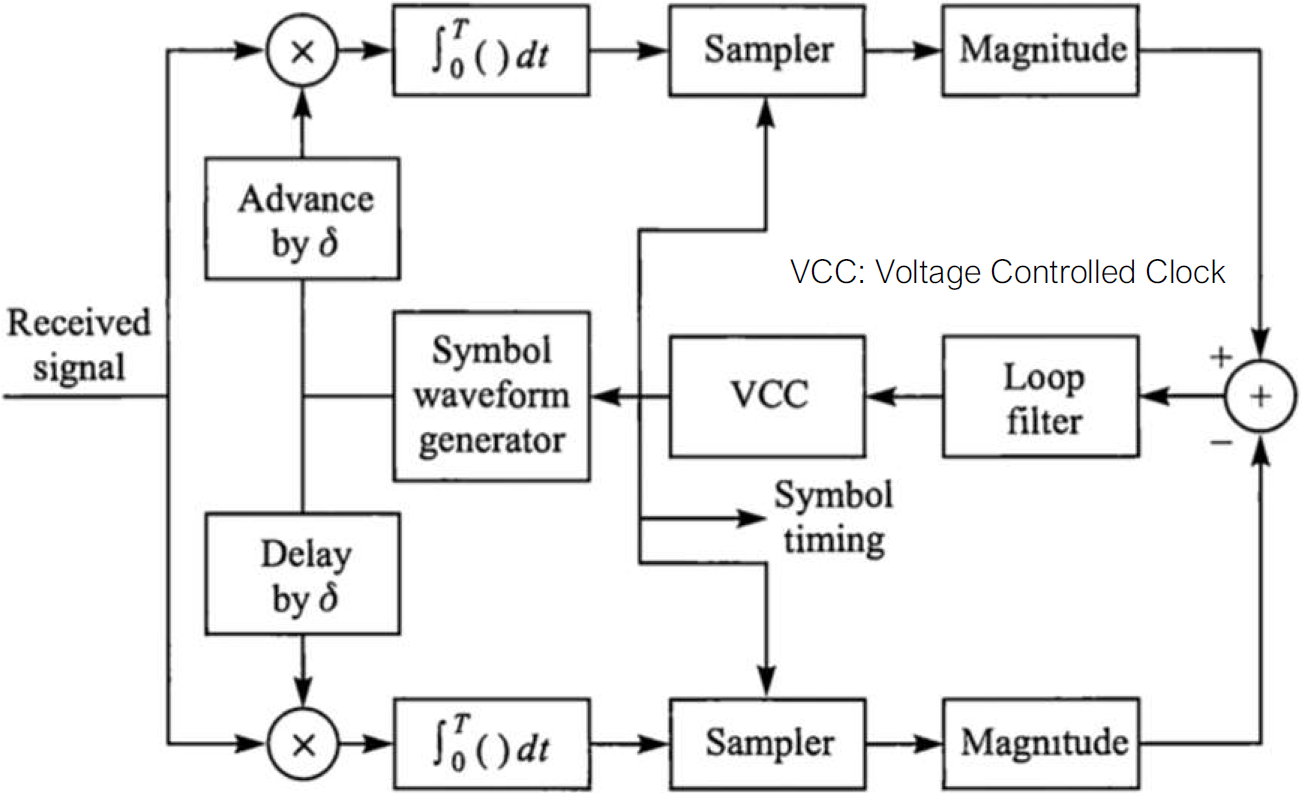
\includegraphics[width=\columnwidth]{images/early_state_synch.png}

\underline{Non decision directed:}

Geting a maximum likelihood on the symbol shape. For example
with a

\underline{Early-late synchronizer}:

We can create a system where we compute the difference between the correlation with shift
$+\delta$ and $-\delta$. If the difference is null we have the optimum otherwise we shift.

The channel can be represented by its transfer function. Equalization is the estimation and application of this
transfer function. This allows to fight ISI. But with OFDM we have long guard intervals that
render equalization unnecessary.
\end{multicols*}

% \subsubsection*{Subsection 2}
% \lipsum[1-10]

\end{document}